\section{C\#2: \slog and \slogxx}


\subsection{Protocols and Implementations}

\slog is one of the latest geo-distributed databases that provides 
strict serializability, and \slog is designed to be deployed 
among a small number of data centers in a full-replication 
manner. \slog lets each data center master a number of shards by 
ordering all transactions accessing these shards, forming a 
``local log'' for each data center. \slog also 
has a global Paxos-based service for ordering all 
transactions accessing shards mastered by multiple data centers,
forming a ``global log''. The global log and local log 
together forms a partial order for all transactions; all data centers 
collect all logs and execute transactions determinstically~\cite{calvin:sigmod12, slog} 
using 2PL according to the partial order. 

However, \slog algorithm is not suitable for partial replication 
as it requires all data centers to hold all shards and collect 
all logs. Directly applying the \slog for partial replication is 
not viable as its 2PL during execution causes not only
extra round trips during, but also creates long blockings if 
data are located in different geographical sites. 

To address this problem, we propose \slogxx by removing 
the heavy cross-datacenter 2PL from \slog, with a much higher performance 
ensuring \xxcons. 
\slogxx inherits the two-level hierarchal ordering approach from
\slog. \slogxx has a global ordering service for the whole system 
and one local ordering service for each region. Transactions accessing 
one single region are directly ordered by its local ordering service, while 
transactions accessing more than one region are first ordered 
by the global ordering service and then dispatched to each accessed region's 
orderer. Each region executes relevant transactions in a one-shot manner 
but does not involve 2PL during execution. 

\begin{figure}[ht]
	\centering
	\subfloat[\footnotesize \slog.]{
	   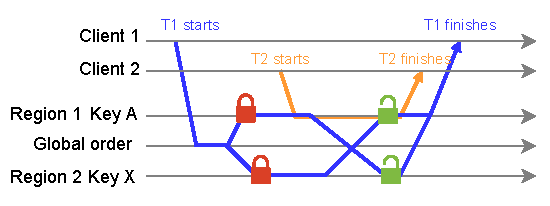
\includegraphics[width=0.45\columnwidth]{figures/slog.pdf}
	   \label{fig:slog}
	}
	\hfill % 在子图之间添加空白空间,确保它们并排排列
	\subfloat[\footnotesize \slogxx]{
		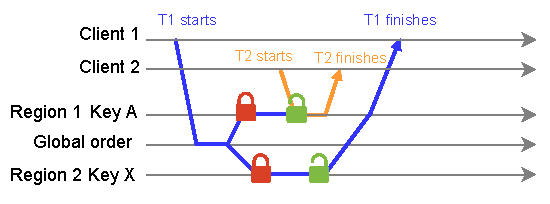
\includegraphics[width=0.45\columnwidth]{figures/slog-rls.pdf}
		\label{fig:slog-rls}
	}
\caption{Comparison of \slog with \slogxx.}
\label{fig:comparison}
\end{figure}




\begin{figure}[t]
	\centering
	\begin{subfigure}[t]{0.49\columnwidth}
	   \centering
  	   \includegraphics[width=\columnwidth]{eval-figs/slogxx-client--tput.pdf}
	   \subcaption{Tput.}
	\end{subfigure}
	\begin{subfigure}[t]{0.49\columnwidth}
		\centering
		\includegraphics[width=\columnwidth]{eval-figs/slogxx-client--lat.pdf}
		\subcaption{Lat.}
	\end{subfigure}
 
\caption{Performance comparison of \slog with \slogxx}.
\end{figure}


\subsection{Evaluation and Discussion}

\clearpage